\chapter{Lösung}
\label{chap:loesung}
% In diesem Kapitel beschreiben Sie Ihre Lösung des Problems. Geben Sie dem Leser genügend Einblick in die Lösung, so dass er Ihre Arbeit entsprechend würdigen kann. Verwenden Sie aber Anhänge für Dinge, die hier nicht unbedingt bis ins letzte Detail verstanden werden müssen.
Die Aufgabenstellung beschreibt das Ziel dieser Arbeit mit dem einfachen Satz "`Ziel dieser Arbeit ist die Entwicklung und Anwendung eines Systems zur Speicherung (von Daten) in einer Semantischen Datenbank..."'.  Dies klingt doch einigermassen simpel, die Autoren sollen also Daten in einem Datenspeicher ablegen. Das einzige unbekannte an dieser Beschreibung, ist die Spezifikation das es sich bei der Datenbank um eine Semantische Datenbank handeln soll. Erst bei genaueren hinsehen wird interessierten Personen bewusst, das sich einiges dahinter verbirgt. Auf der einen Seite eine Ansammlung von neuen Technologien und Theorien. Auf der anderen Seite eine völlig unbekannte und vorallem ungewohnte Denkweise, welche erst erkannt und dann auch wirklich angewendet werden muss. Dies ist gerade für Personen mit Informatik, speziell Objektorientiertem Hintergrund eine echte Herausforderung. Die Erfahrungen und Schwierigkeiten dabei werden im Kapitel Vorgehen - Modellierung \ref{sub:modellierung_der_ontologie} beschrieben.

Eine weitere Anforderung, welche bei der spezifikation der Milestones erstaunlicherweise in den Hintergrund gedrängt wurde, ist der Anspruch der Autoren fähig zu sein, innerhalb einer gewissen Wissensdomäne Fragen zu beantworten. Das klingt schon ein bisschen komplizierter, da im ersten Abschnitt deutlich gemacht wurde, dass die ganze Arbeit auf der Basis von Semantik aufgebaut werden soll. 

Die Organisation sowie die Herangehensweise der Autoren wurden im Kapitel Administratives\ref{chap:administratives} und Vorgehen\ref{chap:vorgehen} ausführlich beschrieben. In diesem Kapitel liegt der Fokus auf der tatsächlichen Lösung der Anforderungen.


\section{Von der Wissenserarbeitung zum Tutorial}
\label{sec:loesung_tutorial}
Um die oben erwähnten Technologien, Sprachen und Theorien zu erarbeiten und diese vorallem mit dem Leser zu teilen wurde ein Tutorial erarbeitet. Bei dieser Teillösung war ein schwieriger Part die Gratwanderung ein einfach nutzbares Tutorial zu erstellen, dem Benutzer aber auch genügend Hintergrundwissen zu vermitteln, so das er wirklich verstehen kann was hinter hinter einer Wissensmodellierung respektive eines Expertenssystems steckt. Daraus entstand ein Dokument, welcher die Modellierung aus drei Aspekten beleuchtet. Diese werden bereits im Kapitel Vorgehen \ref{subsec:dokumentation_wissensmodellierung_aufbau} beschrieben.

\section{Modellierung}
\label{sec:loesung_modellierung}

Semantische Datenbanken werden auf Basis von Ontologien gebildet. Eine Ontologie wird für eine Problemdomäne abgebildet und bildet ihr Wissen ab. Die Problemdomäne dieser Arbeit ist das Reisen. Speziell wurde entschieden sich vorerst auf Ausflüge in der Schweiz zu begrenzen. Damit ist es möglich die Mächtigkeit eines Expertensystems aufzuzeigen. Die gesamte Modellierung wird mithilfe von OWL formuliert. bei OWL handelt es sich um eine Ontologieabbildungssprache. Benötigte Regeln werden in SWRL formuliert. Details dazu können im Tutorial nachgelesen werden. TODO ref zu Tutorial

Zur Veranschaulichung wurde jeder Teil der Ontologie und die dazugehörigen Regeln in einem Semantischen Netz abgebildet. Sämtliche Grafiken finden sich als Anhang TODO.  


\begin{figure}[H]
\centering \rotatebox{0}{\scalebox{0.3}[0.3]{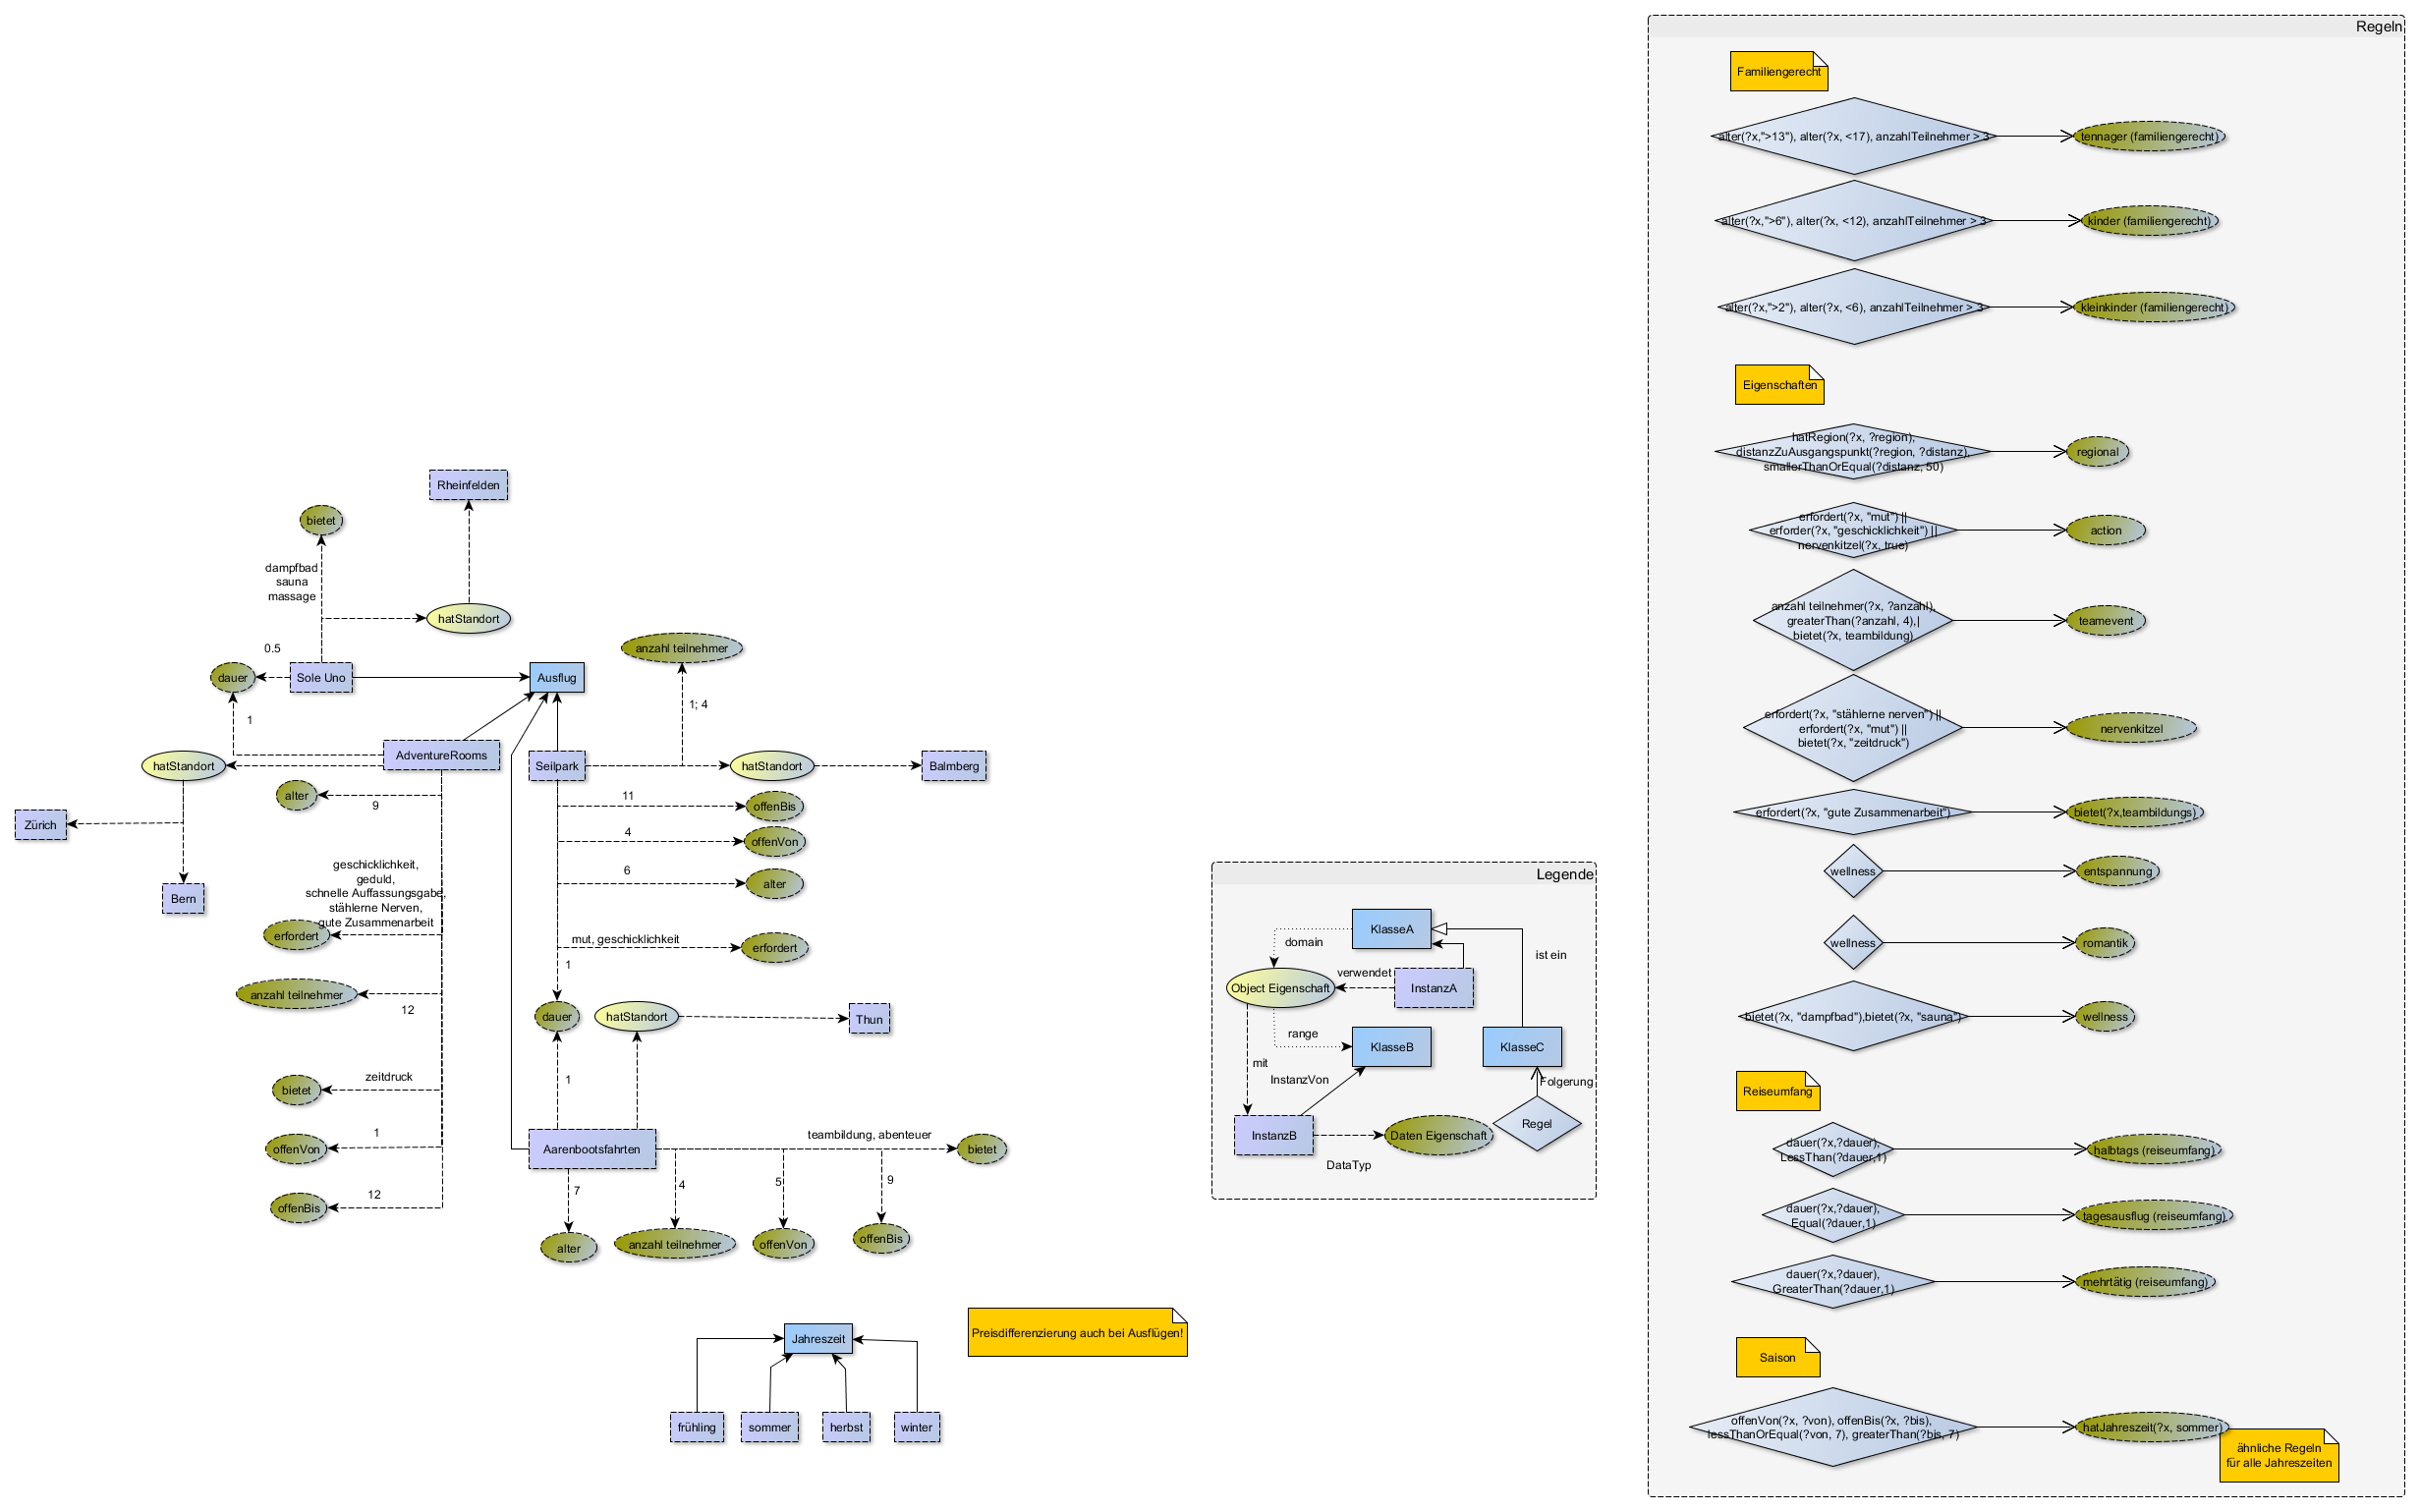
\includegraphics{bilder/semNetzLoesung.png}}}
\caption{Ausschnitt des Semantischen Netzes zur Abbildung der Ontologie.\label{fig:semNetzLoesung}\protect\footnotemark}
\end{figure}
\footnotetext{Eigene Darstellung mittels yEd.}


Durch die Beschränkung der Problemdomäne auf Tages und Wochenendausflüge in der Schweiz konnten zwei Hauptkomponenten (Ausflug und Restaurant) extrahiert werden. 

Sowohl Restaurant als auch Ausflug werden durch "`Bedinungsproperty"' beschrieben. Ein Restaurantbesitzer könnte also den  Betreiber des in dieser Arbeit erzeugten Reiseplaners Qualitäten angeben, welche sein Restaurant ausmacht. Diese Eigenschaften gehen von der Beschreibung des Ambientes, über kulinarischen Spezialitäten zu den durchschnittlichen Preisen welche das Restaurant hat. Der Ausflug ist durch andere Werte wie Anzahl Teilnehmer, Öffnungszeiten, oder was ein Ausflug bietet oder erfordert beschrieben.
Mittels Regeln ist festgelegt welche Folgerungen aus diesen Eigenschaften abgeleitet werden können.

Um die verschiedenen Möglichkeiten beim Abbilden einer Ontologie aufzuzeigen, wurden für die Unterteilung jede der Komponenten eine andere Umsetzung gewählt. Die Klasse Restaurant hat verschiedene Unterklassen. Der Besucher hat also bei der Suche die Auswahl zwischen verschiedenen Typen von Restaurants auszusuchen. Je nach gewähltem Typ müssen unterschiedliche Kriterien (Bedinungspropertys) erfüllt sein. So ist zum Beispiel festgelegt das eine raffinierte Küche mit frischen und saisonalen Speisen auf ein Gourmet Restaurant schliessen lässt. Wenn also in diesem Fall der Benutzer auswählen würde, dass er ein Gourmet Restaurant sucht, würden nur jene Restaurants ermittelt welche als Bedingungsproperty raffinierte mit frischen und saisonalen Speisen aufweisen.  Das Preissemgent ist als Klasse definiert mit Individuen für jedes definierte Segment, wenn der Durchschnittspreis in einem bestimmten Rahmen liegt, definieren Regeln in welchem Preissegment das Restaurant liegt.  Dies ist durch ein ObjectProperty festgelegt. ObjectPropertys beschreiben die Beziehungen zwischen zwei Individuen.\\ 
Bei den Ausflügen werden dem Benutzer des Reiseplaners "`Folgepropertys"' angeboten. Mittels der vorher erwähnten Regeln ist festgelegt welche Bedienungen zutreffen müssen um eine gewisse Eigenschaft zu erfüllen. So ist zum Beispiel festgelegt das ein Ausflug der Wellness bietet entspannt und romantisch ist.\\ Sowohl Folgerungen als auch Bedienungen werden in Form von sogenannten DataPropertys definiert. Diese legen eine Eigenschaft auf ein Individuum fest.

In beiden Fällen ist zu beachten, das der Benutzer sich entscheiden kann ob er entweder eine Region oder Ortabhängige Einschränkung für die Suche festlegen kann. Die Beziehung zwischen den Region/Orten und den konkreten Ausflügen/Restaurants wird mit Hilfe von ObjectPropertys erreicht. Es wird also zum Beispiel gesagt ein Ausflug hat den Standort Bern. Als Erweiterung kann der Benutzer auch nur festlegen, dass er ein Restaurant sucht, welches sich im gleichen Ort respektive in der gleichen Region befindet wie der Ausflug.

Eine Besonderheit von Ausflügen ist, dass sie nicht das ganze Jahr über geöffnet sein können. Durch DataProperty kann der Betreiber festlegen von wann bis wann ein Ausflug geöffnet hat. Dank geeigneter Regeln wird abgeleitet in welcher Saison ein Ausflugziel geöffnet hat. Eines der grösseren Probleme bei der modellierung hat die Zeitbeschränkung ergeben. Bekannterweise kann mit dem perfekten Zeitplaner eine ganze Bachelorthesis gefüllt werden. Da dies in dieser Arbeit nicht der Fokus war, und die Autoren entschieden haben, dass es auch keinen Sinn macht, diese Problematik einfach in Form von Programmlogik zu lösen, fällt die Zeitplanung relativ simpel aus. Es kann festgelegt werden wie viel Zeit ein Ausflug in Anspruch nimmt. Später kann der Benutzer des Reiseplaners angeben wie lang er Zeit hat. Zur Auswahl stehen nur die Kriterien halbtags, ganztags und mehrtägig. In dieser Version des Reiseplaners werden in der Anfrage immer nur jene Ausflüge ausgegeben, welche der festgelegten Zeiteinheit entsprechen.


 
\subsection{Technische Schwierigkeiten}
\label{subsec:loesung_modellierung_technischeSchwierigkeiten}
TODO: evt doch in kapitel Technologien verschieben?!\\
Im Laufe der Modellierung sind die Autoren auf ein für Sie unerklärliches Phänomen gestossen. So war es dem Reasoner in Stardog nicht möglich von einer DataProperty mit einem Wert auf die gleiche DataProperty zu schliessen. Konkret wollten die Autoren aussagen, dass ein Ausflug der eine Sauna bietet auch Wellness bietet. Der Inferenzmaschine von Stardog war es nicht möglich diesen Schluss zu ziehen. Im Entwicklungstool Protégé wurde die Schlussfolgerung aber richtig angezeigt. Nach längeren Recherchen entschieden die Autoren das es sich bei dieser Einschränkung wohl um einen technischen Fehler von Stardog handeln muss. Dies war doch sehr verwirrend, da beide Werkzeuge den gleichen Reasoner (Pellet) verwenden. Nach dem Buckreporing in der Stardogcommunity erhielten die Autoren die Information, dass es sich tatsächlich um einen Fehler im System handelt. Dieser würde mit dem nächsten Realies gefixt. \\
Also Work-Aorunt wurde die Modellierung von den Autoren so umgebaut, dass Wellness ein DataProperty vom Type Boolean ist.

\subsection{Output}
\label{subsec:loesung_modellierung_output}
Ein Teil des Outputs der Modellierung sind die oben erwähnten Semantischen Netze. Diese wurden in drei Grafiken aufgeteilt. Auf der ersten Grafik wird die gesamte Region/Ort Problematik abgebildet. Auf je zwei weiteren Grafiken wurden die Details zu den Restaurants respektive Ausflügen dargestellt.

Der zweite Teil ist ein durch das Entwicklungswerkzeug automatisch generierte RDF \ XML Dokument. Darin ist die Semantische Datenbank mittels owl formal erfasst. Es handelt sich also um die konkreten Daten.

\section{Generieren von Abfragen}
\label{sec:loesung_sparql}

Während die Problemdomäne abgebildet wurde, und für die endgültige Suche mussten immer wieder Abfragen generiert werden. Dies geschieht in einer Semantischen Datenbank mittels sparql Abfragen. Bei Spargl handelt es sich um eine  Abfragesprache für Ontologien todo ref Tutorial. Die Abfragen sind als ein Teil des Resultats in der Benutzeroberfläche integriert. So konnte verhindert werden, dass der Leser der Arbeit gezwungen ist, sich die Sprache anzueignen um die Suche zu benutzten.


\section{Benutzeroberfläche}
\label{sec:gui}

Nun sind alle oben beschriebenen Anforderungen abgedeckt. Eine letzte Aufgabe, die bis zu diesem Punkt noch unterschlagen wurde lautet "`...Besondere Bedeutung kommt dabei der Schnittstelle zwischen Mensch und System zu..."'. Nachdem klar wurde, dass es in keiner weise Benutzerfreundlich ist, Abfragen mittels Sparql selber zu schreiben, haben die Autoren entschieden eine Benutzeroberfläche zu implementieren. Dabei wird der Benutzer des Reiseplaners mit Hilfe eines Assistenten durch die Auswahl geführt. Neben der Vermeidung von Sparql während der Benutzung, ist so sichergestellt das der Benutzer nur Abfragen stellen kann, welche wenigstens in der theorie Sinn ergeben. 
In einem ersten Schritt kann der Besucher entscheiden ob er nur ein Ausflug planen will, oder auch nach einem Restaurant sucht. Im zweiten Schritt werden sämtliche Folgepropertys zu den gewählten Komponenten angeboten. Zum Schluss erhält der Benutzer eine Liste sämtlicher Ergebnisse. Dabei wird aus allen gewählten Folgepropertys dynamisch eine Sparqlabfrage generiert. In der Outputliste sind der Name des Ausflugs, sein Standort und wenn vorhanden seine URL aufgelistet. Je nach Kriterienliste ist es natürlich möglich, dass keine Reise gefunden wird. Dies ist der Fall, wenn keine der erfassten Reisen auf die gewählten Kriterien passt. Da nur sehr exemplarisch Reisen erfasst wurde ist das Risiko für eine leere Antwort relativ hoch.

TODO: wo wollen wir die Architektur unsere Bentuezroberfläche hinmachen?

